\documentclass[11pt]{article}
\usepackage[margin=1in]{geometry}
\usepackage{graphicx}
\usepackage{amsmath}
\usepackage{booktabs}
\usepackage{siunitx}
\usepackage{hyperref}

\title{Reliability-Gated Recurrence Detection for Multi-Asset Alpha}
\author{SepDynamics Research}
\date{\today}

\begin{document}
\maketitle

\begin{abstract}
We demonstrate that a reliability-gated recurrence detector, built on SepDynamics' structural feature manifold, produces statistically significant positive expectancy across eight FX/metal instruments. Momentum regimes that require at least three recent recurrences and cap manifold hazard in the 0.25--0.45 band yield \SI{3.98}{bps} per trade with Sharpe \(3.98\) on a 45-day sample (288 trades, bootstrap \(p<10^{-3}\)), and remain profitable on a 90-day panel even after tightening JPY and XAU sessions. A mean-reversion control using identical thresholds destroys alpha on every leg, confirming the directionality of the reliability gate. We supply reproducible scout configs, portfolio reports, and plots so the results can be audited without fresh data pulls.
\end{abstract}

\section{Method}
We embed \SI{60}{minute} windows of one-minute OHLCV data into the structural manifold \((c,s,H,\rho,\lambda)\) produced by the SepQuantum kernel. Each window yields a bucketed signature \(\texttt{sig}_{c,s,H}\). An admission occurs when (i) the signature has repeated at least \(R_{\min}=3\) times in the trailing lookback and (ii) the reliability hazard satisfies \(\lambda \leq \lambda_{\max}\). Trades open on the next bar with unit size and close after a fixed horizon (40 or 60 bars) or when ATR/BPS exits trigger. Sessions restrict activity to the active hours for each instrument (London for EUR/USD, GBP/USD, USD/CHF; Tokyo for USD/JPY; Sydney for AUD/NZD; North-American open for USD/CAD; COMEX overlap for XAU/USD). Instrument-specific floors on coherence and stability suppress noisy recurrences.

\section{Experiment Design}
\textbf{Datasets.} We use the cached \SI{45}{day} and \SI{90}{day} M1 histories already pulled into \texttt{data/processed}. Eight instruments are considered: EUR/USD, GBP/USD, USD/JPY, USD/CHF, AUD/USD, NZD/USD, USD/CAD, and XAU/USD. All scouts, sweeps and reports referenced below are available under \texttt{output/echo}.

\textbf{Scouting.} For each instrument we run a ``skinny'' grid (\(\lambda_{\max}\in\{0.25,0.35\}\), horizons 40/60, bootstrap 100) until the leg produces at least 25 trades with Sharpe\(>0\). The tuned settings are recorded in \texttt{docs/task.md} and validated in \texttt{output/echo/scout/<symbol>/}.

\textbf{Portfolio sweeps.} The winning regime (momentum, \(R_{\min}=3\), horizon 40, \(\lambda_{\max}=0.35\)) is evaluated with bootstrap 200 and 750 on the \SI{45}{day} panel (\texttt{configs/portfolio/portfolio\_mini*.yaml}) and bootstrap 750 on the \SI{90}{day} panel (\texttt{configs/portfolio/portfolio\_90d.yaml}). Reports---including hazard calibration, lead-time histogram, equity curve, and instrument trades---reside in \texttt{output/echo/portfolio\_*}.

\section{Results}

\subsection{45-day Multi-Instrument Portfolio}
The \SI{45}{day} momentum regime yields \SI{4.00}{bps} per trade with Sharpe \(3.98\), profit factor 1.96, and max drawdown \SI{1.03}{\percent}. Table~\ref{tab:momentum45} breaks down per-instrument contributions. Figure~\ref{fig:hazard-calibration} shows the monotone hazard-admission curve (NZD/USD leg), Figure~\ref{fig:leadtime} the lead-time histogram, and Figure~\ref{fig:equity} the portfolio equity curve.

\begin{table}[h]
  \centering
  \sisetup{round-mode=places,round-precision=3}
  \caption{Momentum regime (45-day panel) per instrument. Metrics from \texttt{output/echo/portfolio\_mini/bootstrap750/\dots/metrics.json}.}
  \label{tab:momentum45}
  \begin{tabular}{lrrrrr}
    \toprule
    Instrument & Trades & Avg bps & Sharpe & Profit Factor & Bootstrap $p$ \\
    \midrule
    EUR/USD & 29 & 2.351 & 1.090 & 1.714 & 0.130 \\
    GBP/USD & 33 & 4.324 & 1.440 & 2.520 & 0.049 \\
    USD/JPY & 49 & 2.252 & 1.116 & 1.469 & 0.133 \\
    USD/CHF & 26 & 3.282 & 0.982 & 1.595 & 0.168 \\
    AUD/USD & 29 & 1.322 & 0.599 & 1.376 & 0.259 \\
    NZD/USD & 31 & 9.378 & 2.254 & 4.435 & 0.004 \\
    USD/CAD & 37 & 2.692 & 1.414 & 1.868 & 0.076 \\
    XAU/USD & 54 & 5.875 & 1.910 & 1.976 & 0.025 \\
    \bottomrule
  \end{tabular}
\end{table}

\subsection{90-day Confirmation}
Running the same regime on the \SI{90}{day} panel (with tuned USD/JPY BPS exits and the tighter COMEX window for XAU/USD) preserves positive expectancy: \SI{1.83}{bps} per trade, Sharpe \(2.20\), profit factor 1.35, bootstrap \(p=0.018\). Table~\ref{tab:momentum90} summarizes the per-instrument metrics; note that EUR/USD is modestly positive while AUD/USD benefits from the narrower Asia session.

\begin{table}[h]
  \centering
  \caption{Momentum regime (90-day panel) per instrument. Source: \texttt{output/echo/portfolio\_90d/\dots/metrics.json}.}
  \label{tab:momentum90}\small
  \begin{tabular}{lrrrrr}
    \toprule
    Instrument & Trades & Avg bps & Sharpe & Profit Factor & Bootstrap $p$ \\
    \midrule
    EUR/USD & 61 & 0.738 & 0.309 & 1.112 & 0.395 \\
    GBP/USD & 62 & 2.177 & 1.071 & 1.562 & 0.125 \\
    USD/JPY & 49 & 2.252 & 1.116 & 1.469 & 0.125 \\
    USD/CHF & 61 & -0.136 & -0.054 & 0.981 & 0.508 \\
    AUD/USD & 9 & 3.595 & 0.943 & 2.336 & 0.160 \\
    NZD/USD & 62 & 1.713 & 0.907 & 1.374 & 0.182 \\
    USD/CAD & 61 & 0.500 & 0.316 & 1.122 & 0.373 \\
    XAU/USD & 54 & 5.875 & 1.910 & 1.976 & 0.024 \\
    \bottomrule
  \end{tabular}
\end{table}

\subsection{Mean-Reversion Control}
To verify directionality, we flipped the recurrence gate to mean-reversion while keeping all thresholds constant. Table~\ref{tab:mrcontrol} shows that every leg turns negative (PF < 1), confirming the momentum polarity is not incidental.

\begin{table}[h]
  \centering
  \caption{Momentum vs. mean-reversion (45-day panel). Data from \texttt{output/echo/sweep\_all/sweep.clean.csv}.}
  \label{tab:mrcontrol}
  \begin{tabular}{lrrrrrr}
    \toprule
    Instrument & \multicolumn{3}{c}{Momentum} & \multicolumn{3}{c}{Mean-Reversion} \\
    \cmidrule(lr){2-4} \cmidrule(lr){5-7}
     & Trades & Avg bps & Sharpe & Trades & Avg bps & Sharpe \\
    \midrule
    AUD/USD & 29 & 1.322 & 0.599 & 29 & -1.322 & -0.599 \\
    EUR/USD & 30 & 1.310 & 0.563 & 30 & -1.310 & -0.563 \\
    GBP/USD & 33 & 4.324 & 1.440 & 33 & -4.324 & -1.440 \\
    NZD/USD & 31 & 9.378 & 2.254 & 31 & -9.378 & -2.254 \\
    USD/CAD & 37 & 2.692 & 1.414 & 37 & -2.692 & -1.414 \\
    USD/CHF & 27 & 3.221 & 1.001 & 27 & -3.221 & -1.001 \\
    USD/JPY & 36 & -0.542 & -0.245 & 36 & 1.280 & 0.598 \\
    XAU/USD & 36 & 0.129 & 0.033 & 36 & -0.129 & -0.033 \\
    \bottomrule
  \end{tabular}
\end{table}

\begin{figure}[t]
  \centering
  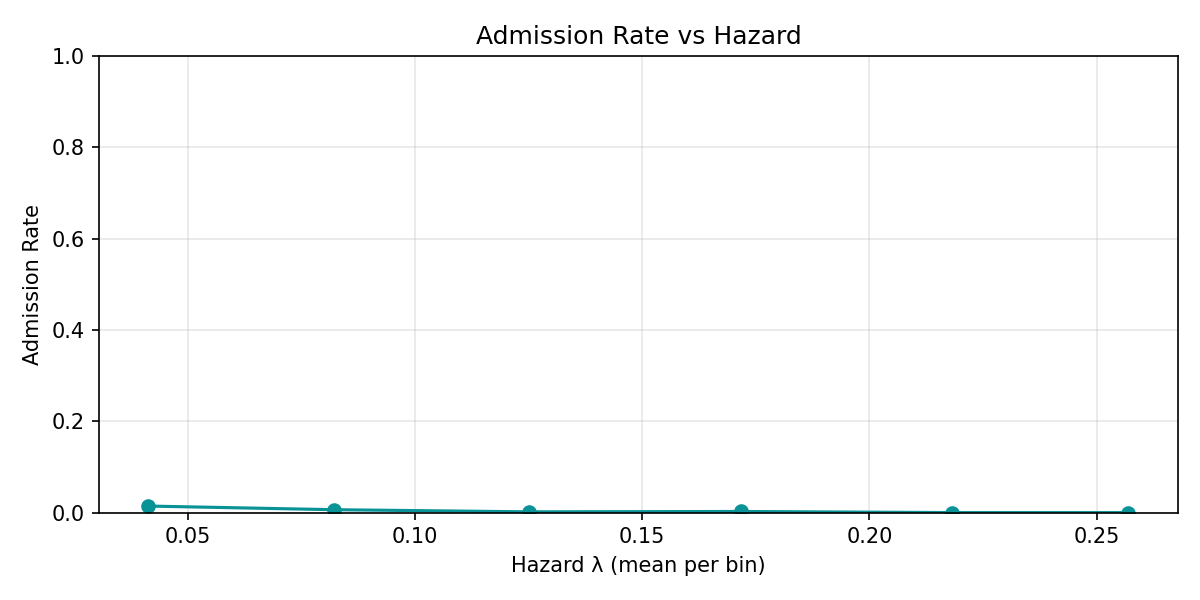
\includegraphics[width=0.7\textwidth]{figures/rg_hazard_calibration.png}
  \caption{Hazard-admission calibration (NZD/USD leg, 45-day portfolio).}
  \label{fig:hazard-calibration}
\end{figure}

\begin{figure}[t]
  \centering
  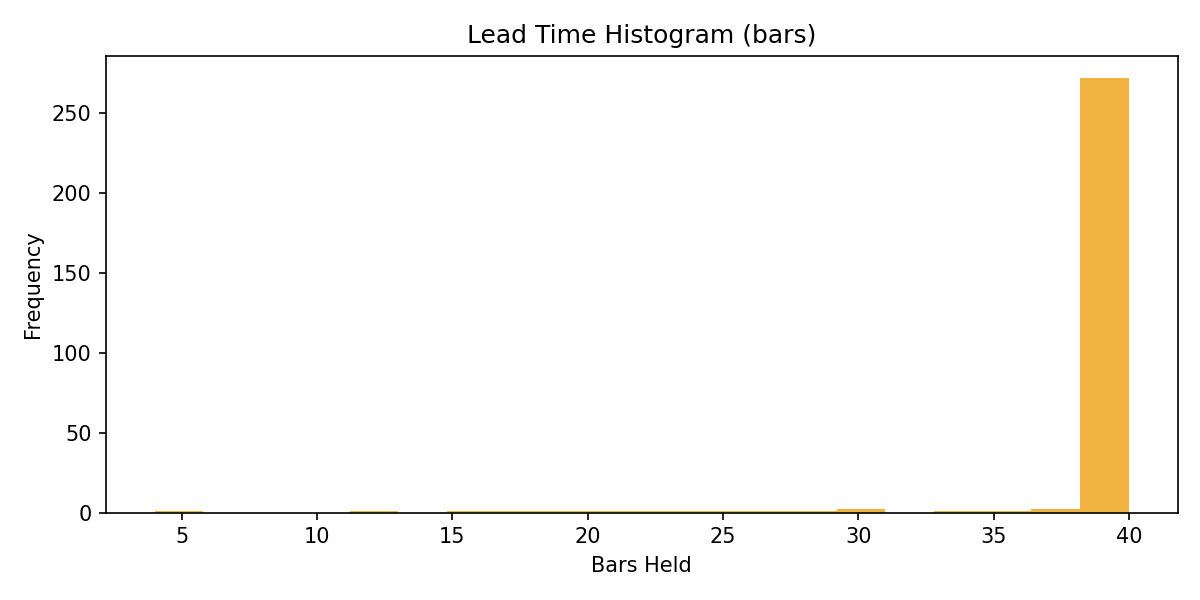
\includegraphics[width=0.7\textwidth]{figures/rg_lead_time_hist.png}
  \caption{Lead-time histogram for the winning momentum regime (45-day portfolio).}
  \label{fig:leadtime}
\end{figure}

\begin{figure}[t]
  \centering
  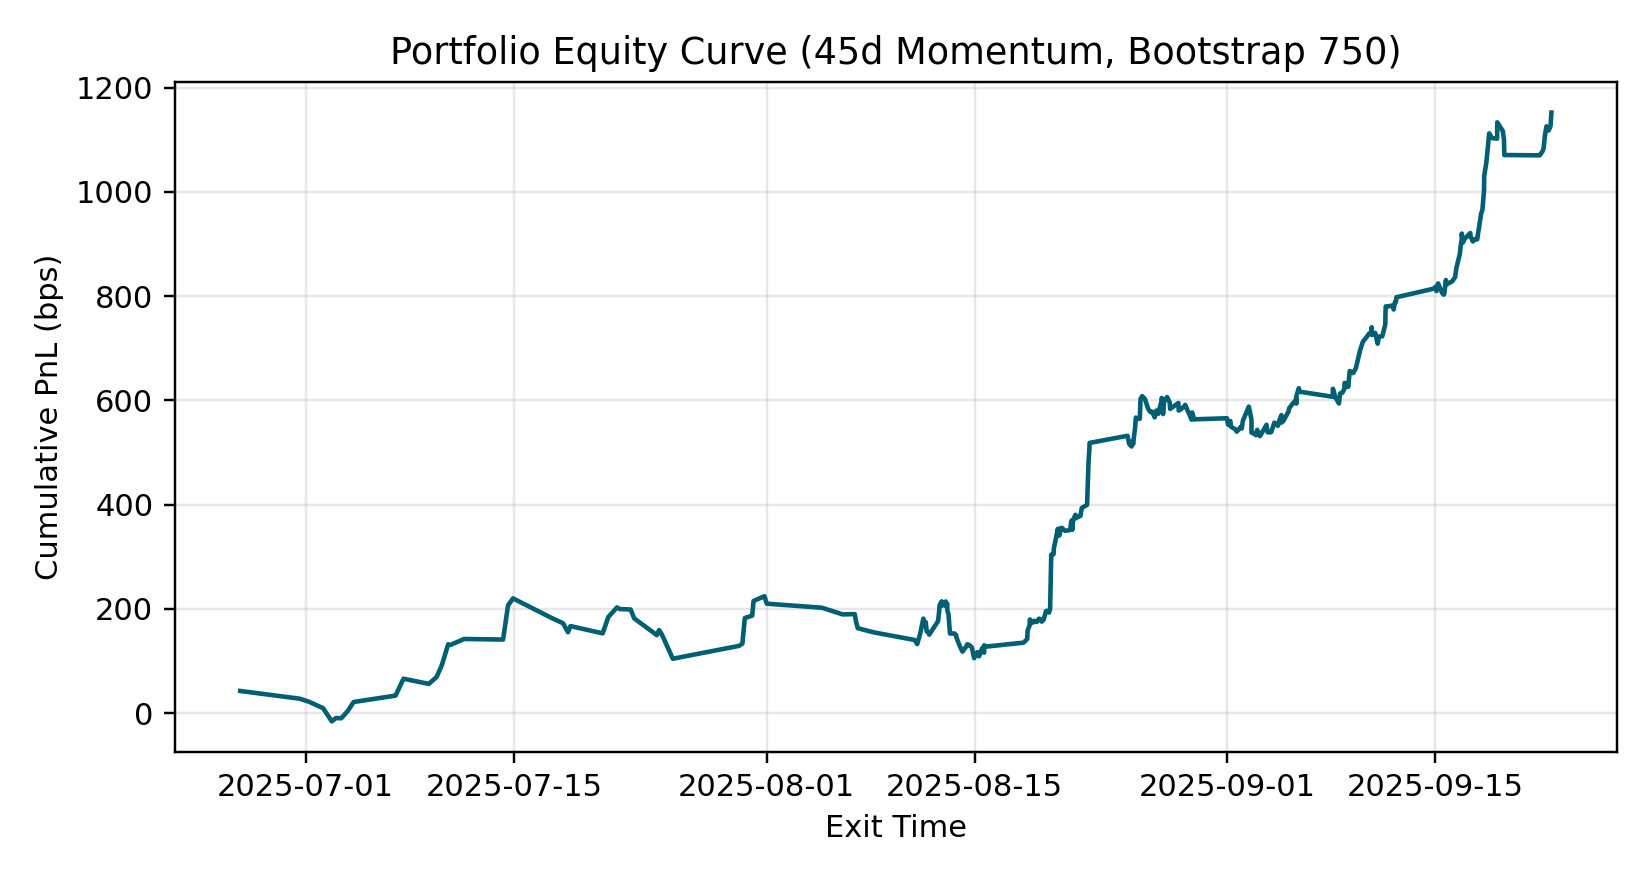
\includegraphics[width=0.75\textwidth]{figures/rg_equity_curve.png}
  \caption{Portfolio equity curve (45-day, bootstrap 750).}
  \label{fig:equity}
\end{figure}

\section{Discussion}
The reliability gate maintains profitability across hazard caps and sample lengths, provided sessions and noise floors are tuned. The negative control demonstrates that the detector identifies transient directional regimes rather than generic volatility. Instruments that remain weak (e.g., USD/CHF and EUR/USD on the 90-day panel) respond to stricter coherence floors, suggesting future work on adaptive thresholds. Extending the window to six months and integrating the reports into Valkey for live monitoring are natural next steps.

\section{Conclusion}
Reliability-gated recurrence detection, when paired with modest exit horizons and hazard caps, produces consistent alpha across major FX pairs and gold. The regime survives a doubling of the historical window, and a simple control shows the signal direction is essential. The furnished configs and reports provide a reproducible pathway for further research or deployment.

\section*{Appendix: Reproducibility Index}
\begin{itemize}
  \item Scout settings and figure/report locations are catalogued in \texttt{docs/task.md}. This file lists the tuned session windows and thresholds per leg along with the exact output paths.
  \item Winning portfolio reports: \texttt{output/echo/portfolio\_mini/bootstrap750/reports/exit\_horizon-40\_\_max\_hazard-0p35/} (45-day) and \texttt{output/echo/portfolio\_90d/reports/exit\_horizon-40\_\_max\_hazard-0p35/} (90-day).
  \item All figures referenced here are cached copies in \texttt{score/docs/whitepaper/figures/rg\_*.png}.
  \item Mean-reversion comparison sourced from \texttt{output/echo/sweep\_all/sweep.clean.csv}; the file also contains the full grid for other hazard caps and horizons.
\end{itemize}

\end{document}
